\section{Source Integrated Simulation Detail}\label{app:source-04}
\noindent\textit{Historical source detail. Several numerical assumptions and design descriptions in this transcription have been superseded by Sections 1--5 and Appendix L. These tables are retained for traceability and are not the current approved mission baseline.}

\noindent\textit{The following is retained from the original project draft for supporting detail and comparison. Numerical claims are preliminary unless specifically reconciled in the main text.}

The Day-in-the-Life (DITL) Simulation represents one of the most
important mission-analysis and systems-engineering activities within the
ANTARA mission framework. The DITL simulation acts as an integrated
operational verification environment used to evaluate whether the
spacecraft can successfully achieve its scientific objectives while
operating within the physical, operational, and resource constraints of
a 3U CubeSat platform.

Unlike isolated subsystem-level analysis, the DITL framework evaluates
the spacecraft as a complete operational system in which orbit dynamics,
spacecraft attitude, power generation, battery charging and discharge,
payload operations, ground-station communications, and mission-mode
transitions all interact simultaneously.

The baseline DITL simulation duration for Mission Concept Review
activities is approximately 12 hours. The team has additionally
completed a year-long simulation using Orekit and Python-based subsystem
models.

The DITL simulation tracks the following operational metrics:

\begin{itemize}
\item
  spacecraft position, velocity, latitude, longitude, altitude, beta
  angle, eclipse status
\item
  Battery energy and SOC, solar array power generation, spacecraft
  electrical load consumption, net power balance
\item
  Attitude error, pointing accuracy, reaction wheel momentum, slew
  events
\item
  SAA detection opportunities, science data volume generated
\item
  Ground-station visibility, contact timing and duration, and cumulative
  data-return volume
\end{itemize}

.

\textbf{Executive takeaways}

\begin{itemize}
\item
  Operationally stable. The spacecraft completes startup detumble,
  repeated science and relay activities, and returns to SUN\_POINTING
  after each activity. SUN\_POINTING occupies 87.5\% of the run.
\item
  Attitude control is accurate outside slews. Steady-state
  95th-percentile pointing and attitude error are both 0.4 deg. The
  larger error peaks are associated with commanded reorientation events.
\item
  Slew execution is well matched to the model. There are 18 slews
  totaling 18.8 minutes. Actual duration differs from the estimate by
  only 0.02 s on average, with a maximum difference of 0.31 s.
\end{itemize}

\textbf{Radiation operations reduce science availability}

The run includes six SAA passes totaling approximately 44.9 minutes.

Across the five proton passes

\begin{itemize}
\item
  Historical detection-conditional sample fraction is approximately 62.7\%; not SAA duration-weighted duty
\item
  The lowest science-active fraction is approximately 37.9\%
\item
  Other passes generally remain between approximately 66\% and 71\%
\end{itemize}

This suggests that the radiation protection logic is active but does not
completely disable science collection during all proton environment.
\begin{figure}[htbp]\centering
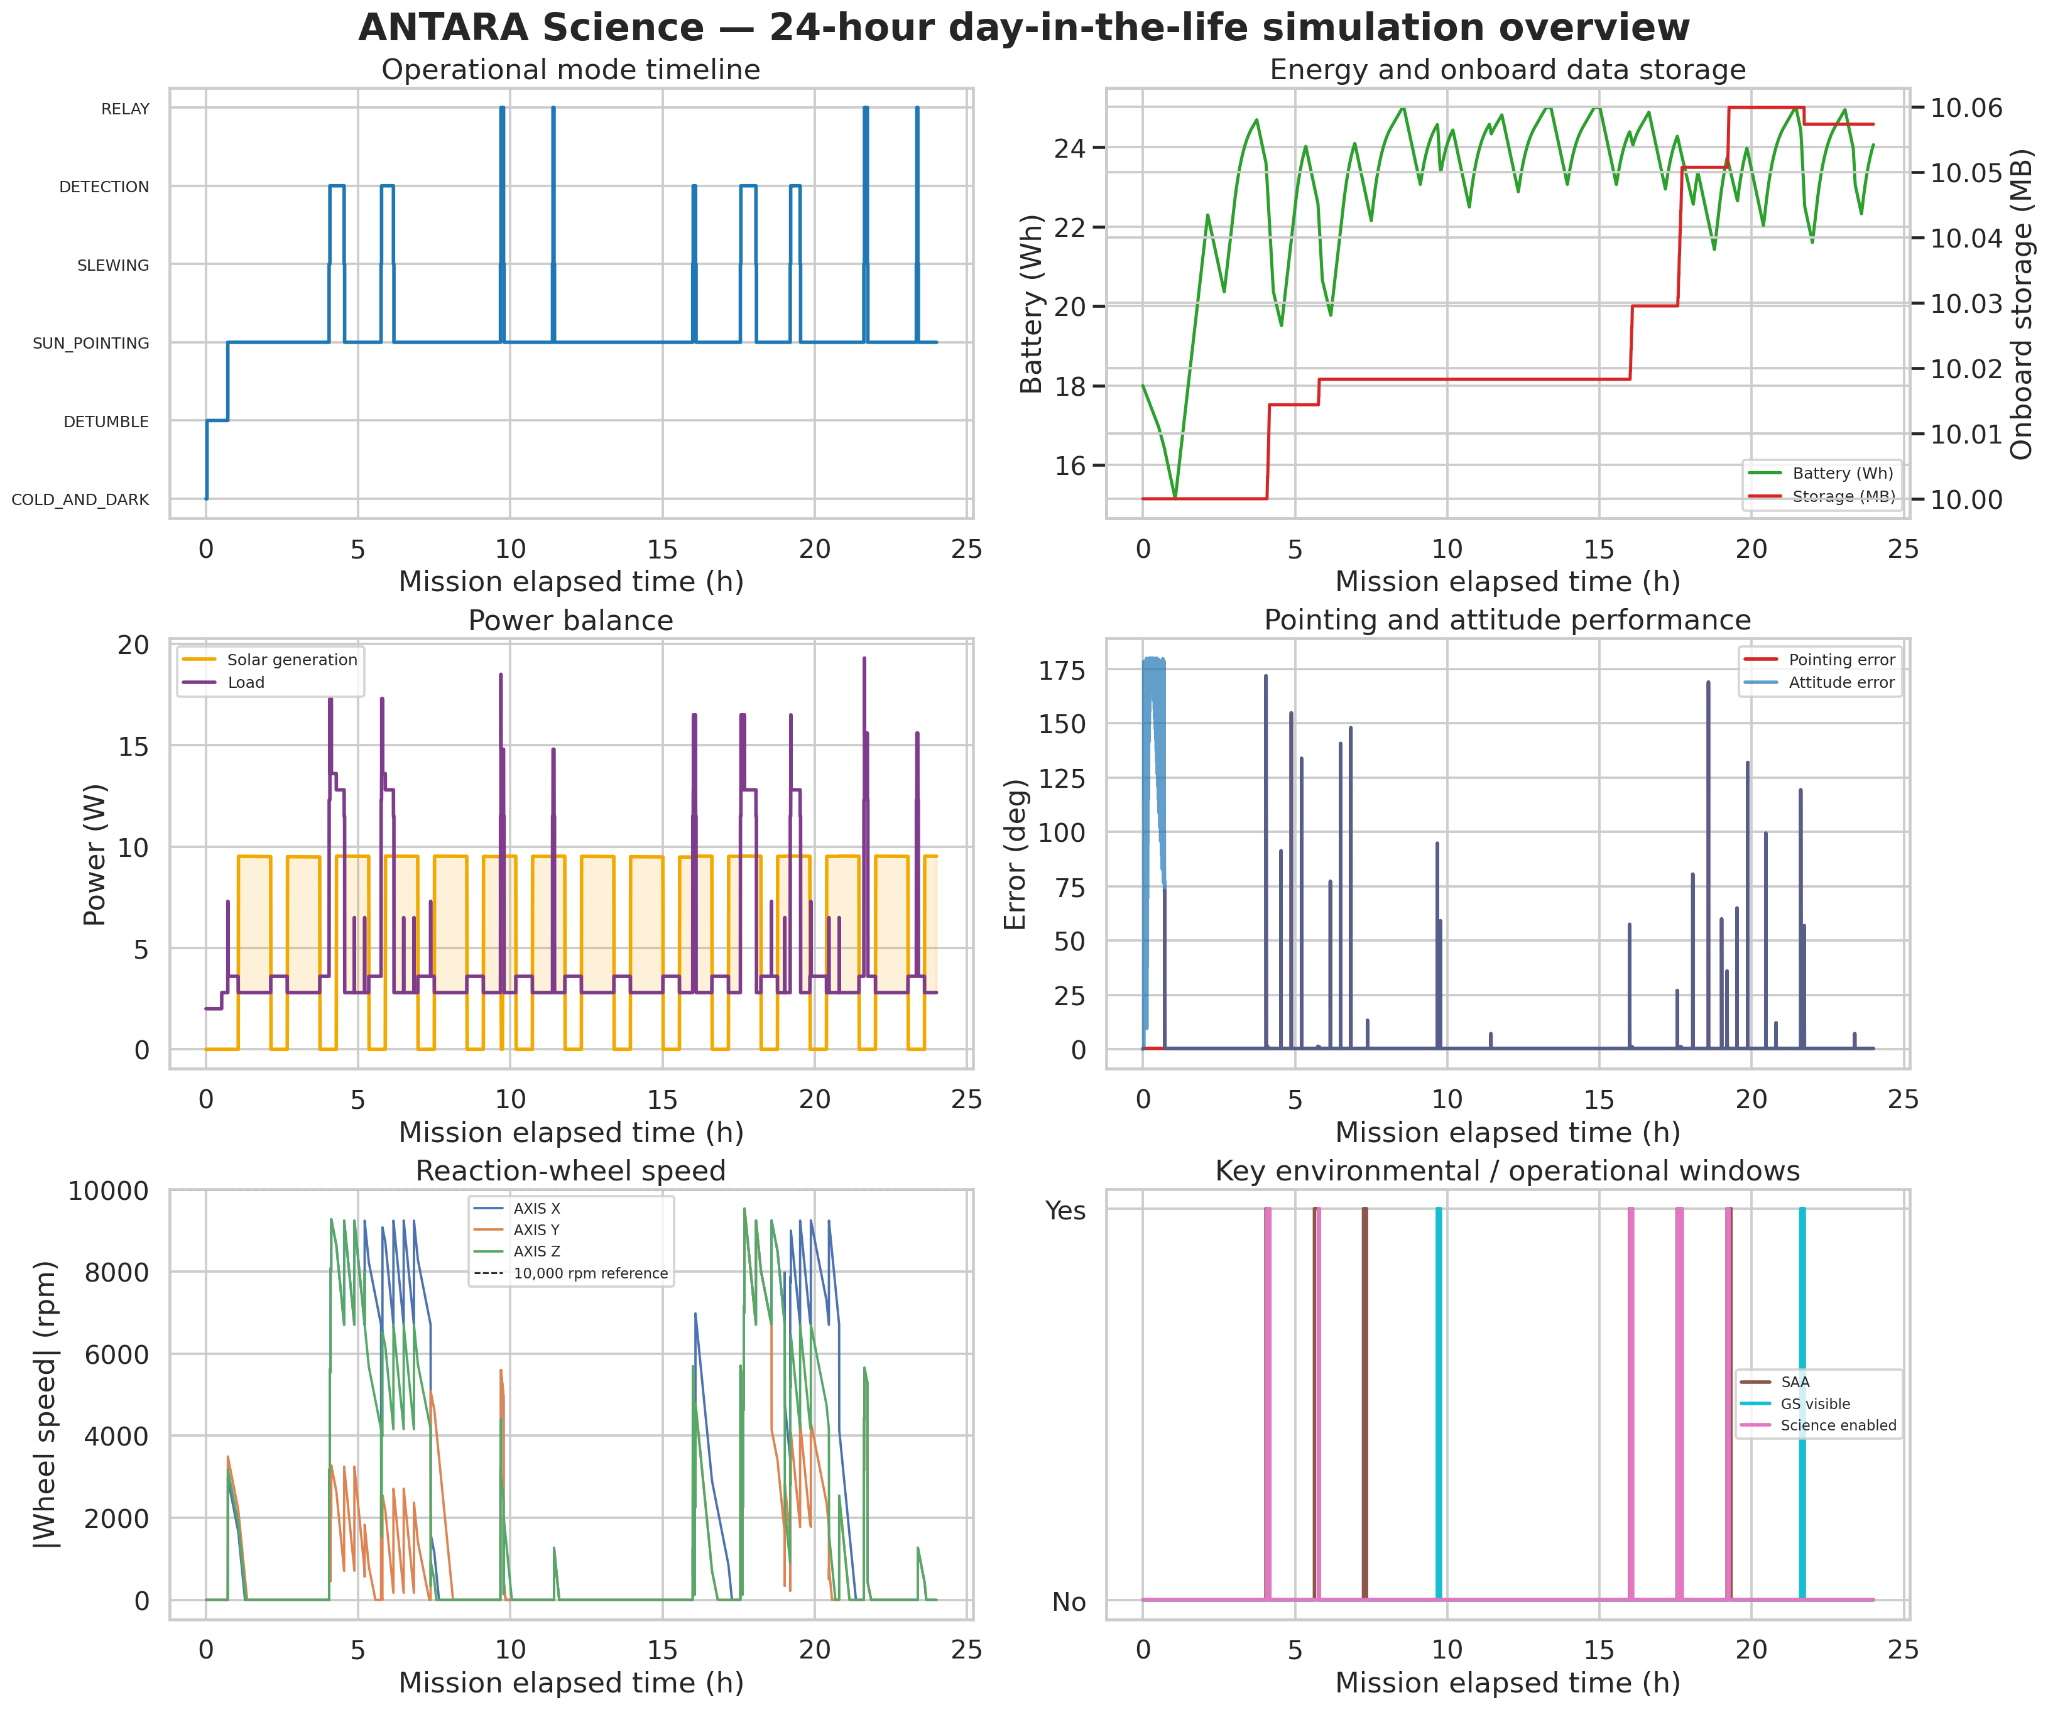
\includegraphics[width=\linewidth,height=0.65\textheight,keepaspectratio]{./media/ditl_overview.png}
\caption{24-hour integrated DITL overview: mode timeline, energy and storage, power, pointing, reaction-wheel speed and operational windows.}\end{figure}


The battery never approaches depletion during this run.

\begin{itemize}
\item
  Initial battery energy is 18.00 Wh
\item
  Minimum battery energy is 15.15 Wh
\item
  Minimum level is approximately 84.2\% of the initial value
\item
  Final battery energy is 24.06 Wh
\item
  Net battery gain over the simulation is approximately 6.06 Wh
\end{itemize}

\textbf{Operational Mode Distribution (24 hours):}

\begin{longtable}{@{}
  >{\raggedright\arraybackslash}p{(\columnwidth - 4\tabcolsep) * \real{0.2991}}
  >{\raggedright\arraybackslash}p{(\columnwidth - 4\tabcolsep) * \real{0.2436}}
  >{\raggedright\arraybackslash}p{(\columnwidth - 4\tabcolsep) * \real{0.4573}}@{}}
\caption{24-hour operational-mode distribution}\\
\toprule\noalign{}
\textbf{Mode} & \textbf{Time Steps} & \textbf{Fraction of Day} \\
Sun Pointing & 37,781 & 87.5\% \\
Detection & 3,134 & 7.3\% \\
Detumble & 1,230 & 2.8\% \\
Slewing & 545 & 1.3\% \\
Relay & 450 & 1.0\% \\
Cold \& Dark & 61 & 0.1\% \\
\midrule\noalign{}
\endhead
\bottomrule\noalign{}
\endlastfoot
\end{longtable}

\textbf{Power and Energy:}

\begin{itemize}
\item
  Average solar generation: 6.05 W
\item
  Minimum battery energy recorded: 15.15 Wh (60.6\% of 25 Wh planning
  capacity)
\item
  No brownouts observed; battery remained above 30\% safety threshold
  throughout the full 24-hour simulation.
\end{itemize}

\textbf{SAA Operations:}

\begin{itemize}
\item
  6 SAA passes observed in 24 hours
\item
  5 of 6 passes achieved active payload science collection
\item
  Total SAA dwell time: \textless2,700 seconds over 24 hours
\item
  Science data generated: 0.060 MB (60 KB) per 24-hour period,
  consistent with 300--400 KB/day (historical estimate, superseded by the v3 sensitivity analysis) estimate at full nominal operations.
\end{itemize}

\textbf{Ground Station Contact:}

\begin{itemize}
\item
  2 contacts with GS1\_India (Goa, 15°N, 74°E) in the 24-hour window
\item
  Contact 1: 368 seconds, maximum elevation 38.5°
\item
  Contact 2: 414 seconds, maximum elevation 77.5°
\item
  Daily downlink capacity at 15--18 kbps (historical, superseded by the ideal 19.2 kbps MCR assumption): \textasciitilde1.5 MB/day ---
  approximately 4× the expected daily science data volume.
\end{itemize}

\textbf{ADCS Performance:}

\begin{itemize}
\item
  Detumble completed in 2,460 seconds from initial body rates of {[}6.0,
  −5.5, 4.5{]} °/s
\item
  18 slew events recorded in 24 hours
\item
  The raw 18-event table gives a minimum slew of 0.442496° (the earlier 5.4° minimum is superseded); the reported maximum is 175.8°; large slews indicate some mode
  transitions require significant attitude manoeuvre time and should be
  factored into operational scheduling.
\end{itemize}

\textbf{Proton Detection (5 active science passes):}

\begin{itemize}
\item
  Historical synthetic FPDU proxy: 50--70\% of the configured AP9-named baseline, not measured detector performance or live AP9
  across all energy channels (5--100 MeV), consistent with partial SAA
  coverage and pitch-angle sampling effects.
\item
  Mean pitch angle ranged 15.6°--77.6° across passes
\item
  Withdrawn count/precision claim: the historical 13,000--108,000 values summed rates without the required time integration. They cannot establish counts or mission-tier precision.
\end{itemize}

\textbf{One-Year Extended Simulation (RAAN 180° baseline):}

\begin{longtable}{@{}
  >{\raggedright\arraybackslash}p{(\columnwidth - 8\tabcolsep) * \real{0.2500}}
  >{\raggedright\arraybackslash}p{(\columnwidth - 8\tabcolsep) * \real{0.1667}}
  >{\raggedright\arraybackslash}p{(\columnwidth - 8\tabcolsep) * \real{0.1282}}
  >{\raggedright\arraybackslash}p{(\columnwidth - 8\tabcolsep) * \real{0.1282}}
  >{\raggedright\arraybackslash}p{(\columnwidth - 8\tabcolsep) * \real{0.3269}}@{}}
\caption{Historical standalone campaign statistics; not verified annual integrated Science output}\\
\toprule\noalign{}
\textbf{Metric} & \textbf{Mean} & \textbf{Min} & \textbf{Max} & \textbf{99\% CI} \\
Average Power (W) & 11.22 & 11.19 & 11.25 & 11.16--11.27 \\
Average SOC & 0.987 & 0.986 & 0.987 & 0.986--0.987 \\
Minimum SOC & 0.834 & 0.834 & 0.834 & 0.834--0.834 \\
Battery Cycles & 787 & 785 & 789 & 783--791 \\
\midrule\noalign{}
\endhead
\bottomrule\noalign{}
\endlastfoot
\end{longtable}
